%% Full-width two-panel diagnostic plot: Outcome supervision tracks the state-only marginal prior across 20 (n, |Sigma|) tasks while exact executor achieves 100%.
\definecolor{stepc}{HTML}{0072B2}\definecolor{outc}{HTML}{D55E00}\definecolor{theoc}{HTML}{009E73}
\definecolor{mutedc}{HTML}{6E6E6E}\definecolor{errc}{HTML}{E59872}
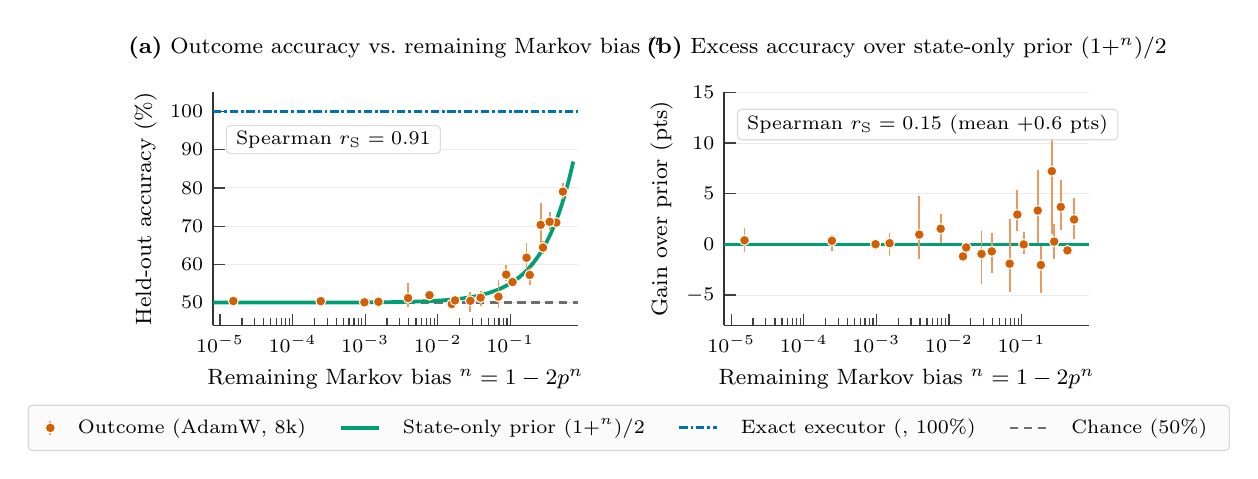
\begin{tikzpicture}
\pgfplotsset{
  every axis/.style={
    scale only axis,
    clip=false,
    width=0.382\textwidth,
    height=2.96cm,
    axis line style={black!80, line width=0.55pt},
    tick style={black!75, line width=0.45pt},
    tick label style={font=\scriptsize},
    label style={font=\footnotesize},
    ylabel style={yshift=-2pt},
    xlabel style={yshift=1pt},
    title style={font=\footnotesize, at={(0.5,1.03)}, anchor=south},
    axis x line*=bottom,
    axis y line*=left,
    ymajorgrids,
    major grid style={black!8, line width=0.35pt}
  },
  every axis plot/.append style={line width=1.05pt}
}

% (a) Held-out outcome accuracy vs remaining Markov bias \lambda^n
\begin{semilogxaxis}[
  name=pb,
  title={\textbf{(a)} Outcome accuracy vs.\ remaining Markov bias $\mixrate^n$},
  xlabel={Remaining Markov bias $\mixrate^n = \lvert 1 - 2p\rvert^n$},
  ylabel={Held-out accuracy (\%)},
  xmin=8e-6, xmax=0.85,
  xtick={1e-5,1e-4,1e-3,1e-2,1e-1},
  ymin=44, ymax=105,
  ytick={50,60,70,80,90,100},
  yticklabels={$50$,$60$,$70$,$80$,$90$,$100$},
  legend style={
    at={(1.14,-0.34)},
    anchor=north,
    legend columns=4,
    font=\scriptsize,
    draw=black!16,
    fill=black!1.5,
    rounded corners=1.5pt,
    inner xsep=6pt,
    inner ysep=2.8pt,
    column sep=6pt,
    cells={anchor=west},
    /tikz/every even column/.append style={column sep=10pt}
  },
  legend image code/.code={
    \draw[#1] (0cm,0cm) -- (0.48cm,0cm);
  }
]
  % Reference baselines & analytical state-only prior
  \addplot[stepc, densely dashdotted, line width=1.05pt, domain=8e-6:0.85, samples=2, forget plot] {100};
  \addplot[mutedc, densely dashed, line width=0.85pt, domain=8e-6:0.85, samples=2, forget plot] {50};
  \addplot[theoc, solid, line width=1.35pt, domain=8e-6:0.74, samples=200, forget plot] {50*(1+x)};

  % Empirical 20-cell AdamW outcome evaluations (exact coordinates)
  \addplot[
    only marks,
    mark=*, mark size=1.8pt,
    mark options={solid, fill=outc, draw=white, line width=0.38pt},
    error bars/.cd, y dir=both, y explicit,
    error bar style={outc!62, line width=0.65pt}, error mark=none,
    /pgfplots/legend image code/.code={
      \draw[outc!62, line width=0.65pt] (0.24cm,-0.09cm) -- (0.24cm,0.09cm);
      \filldraw[fill=outc, draw=white, line width=0.38pt] (0.24cm,0cm) circle[radius=1.8pt];
    }
  ] coordinates {(0.015625,49.6) += (0,0.1) -= (0,0.1) (0.0877915,57.33) += (0,2.467) -= (0,1.633) (0.262144,70.33) += (0,5.667) -= (0,6.233) (0.531441,79.03) += (0,2.167) -= (0,1.933) (0.00390625,51.17) += (0,3.833) -= (0,2.367) (0.0390184,51.27) += (0,1.833) -= (0,2.167) (0.167772,61.73) += (0,3.967) -= (0,3.233) (0.430467,70.93) += (0,0.6667) -= (0,0.5333) (0.000976562,50.07) += (0,0.3333) -= (0,0.5667) (0.0173415,50.57) += (0,0.4333) -= (0,0.8667) (0.107374,55.37) += (0,1.233) -= (0,0.9667) (0.348678,71.13) += (0,2.667) -= (0,2.233) (0.000244141,50.37) += (0,0.5333) -= (0,0.9667) (0.00770735,51.93) += (0,1.467) -= (0,1.433) (0.0687195,51.53) += (0,4.367) -= (0,2.833) (0.28243,64.4) += (0,1.7) -= (0,1.7) (1.52588e-05,50.4) += (0,1.2) -= (0,1.1) (0.00152244,50.2) += (0,1) -= (0,1.3) (0.0281475,50.47) += (0,2.233) -= (0,2.967) (0.185302,57.23) += (0,1.867) -= (0,2.733)};
  \addlegendentry{Outcome (AdamW, $8$k)}

  \addlegendimage{theoc, solid, line width=1.35pt}
  \addlegendentry{State-only prior $(1{+}\mixrate^n)/2$}

  \addlegendimage{stepc, densely dashdotted, line width=1.05pt}
  \addlegendentry{Exact executor ($\thout$, $100\%$)}

  \addlegendimage{mutedc, densely dashed, line width=0.85pt}
  \addlegendentry{Chance ($50\%$)}

  \node[anchor=north west, font=\scriptsize, draw=black!14, fill=white, fill opacity=0.92, text opacity=1, rounded corners=1.5pt, inner xsep=3.5pt, inner ysep=2pt] at (rel axis cs:0.035,0.86) {Spearman $r_{\mathrm S} = 0.91$};
\end{semilogxaxis}

% (b) Excess accuracy over state-only prior (zoomed to [-8, +15] pts)
\begin{semilogxaxis}[
  name=pc,
  at={(pb.east)}, anchor=west, xshift=1.86cm,
  title={\textbf{(b)} Excess accuracy over state-only prior $(1{+}\mixrate^n)/2$},
  xlabel={Remaining Markov bias $\mixrate^n = \lvert 1 - 2p\rvert^n$},
  ylabel={Gain over prior (pts)},
  xmin=8e-6, xmax=0.85,
  xtick={1e-5,1e-4,1e-3,1e-2,1e-1},
  ymin=-8, ymax=15,
  ytick={-5,0,5,10,15}
]
  % Zero-gain state-only prior line
  \addplot[theoc, solid, line width=1.3pt, domain=8e-6:0.85, samples=2] {0};

  % Exact 20-cell residuals and error bars
  \addplot[
    only marks,
    mark=*, mark size=1.8pt,
    mark options={solid, fill=outc, draw=white, line width=0.38pt},
    error bars/.cd, y dir=both, y explicit,
    error bar style={outc!62, line width=0.65pt}, error mark=none
  ] coordinates {(0.015625,-1.181) += (0,0.1) -= (0,0.1) (0.0877915,2.944) += (0,2.467) -= (0,1.633) (0.262144,7.226) += (0,5.667) -= (0,6.233) (0.531441,2.461) += (0,2.167) -= (0,1.933) (0.00390625,0.9714) += (0,3.833) -= (0,2.367) (0.0390184,-0.6843) += (0,1.833) -= (0,2.167) (0.167772,3.345) += (0,3.967) -= (0,3.233) (0.430467,-0.59) += (0,0.6667) -= (0,0.5333) (0.000976562,0.01784) += (0,0.3333) -= (0,0.5667) (0.0173415,-0.3004) += (0,0.4333) -= (0,0.8667) (0.107374,-0.002042) += (0,1.233) -= (0,0.9667) (0.348678,3.699) += (0,2.667) -= (0,2.233) (0.000244141,0.3545) += (0,0.5333) -= (0,0.9667) (0.00770735,1.548) += (0,1.467) -= (0,1.433) (0.0687195,-1.903) += (0,4.367) -= (0,2.833) (0.28243,0.2785) += (0,1.7) -= (0,1.7) (1.52588e-05,0.3992) += (0,1.2) -= (0,1.1) (0.00152244,0.1239) += (0,1) -= (0,1.3) (0.0281475,-0.9407) += (0,2.233) -= (0,2.967) (0.185302,-2.032) += (0,1.867) -= (0,2.733)};

  \node[anchor=north west, font=\scriptsize, draw=black!14, fill=white, fill opacity=0.92, text opacity=1, rounded corners=1.5pt, inner xsep=3.5pt, inner ysep=2pt] at (rel axis cs:0.035,0.93) {Spearman $r_{\mathrm S} = 0.15$ (mean $+0.6$ pts)};
\end{semilogxaxis}
\end{tikzpicture}
